\documentclass[12pt]{scrartcl}

\usepackage[utf8]{inputenc}
\usepackage[naustrian]{babel}
\usepackage{caption}
\usepackage{graphicx}
\usepackage{verbatim}
\usepackage[T1]{fontenc}
\usepackage{lmodern}
\usepackage{subcaption}
\usepackage{amsmath}
\usepackage{amsfonts}
\usepackage{listings}
\usepackage{float}
\usepackage{tikz}
\usepackage{bookmark}

%pdfs
\usepackage{pdfpages}
\usepackage{tikz}

%page borders
\usepackage{geometry}
\geometry{left=2.5cm,right=2.5cm,top=3cm,bottom=2.5cm}

\usepackage{minted}
\setminted {
	%style=igor, %borland, autumn, vs
	encoding=utf-8,
	autogobble,
	tabsize=4,
	linenos,
	breaklines,
	%escapeinside=||
	%bgcolor=bg
	frame=single
}

\newenvironment{code}{\captionsetup{type=listing}}{}

%title/footer/header values
\usepackage{titling}
\title{SWE Zusammenfassung}
\author{Elias Leonhardsberger}
\date{\today{}, Hagenberg}

%footer/header
%\usepackage[automark]{scrpage2}
%\pagestyle{headings}
%\clearscrheadfoot
%\ihead{\thetitle}
%\chead{\theauthor}
%\ohead{\today}
%\cfoot{Seite \pagemark}

\begin{document}
\maketitle
\tableofcontents

\pagebreak

\section{C++}
\subsection{Standard Library}
Der Namensraum \emph{std} ist für die Standardbibliothek von C++ und C reserviert.
Alle C Header-Dateien sind in C++ verfügbar, ihr Name ist immer mit einem \emph{c}
vorangestellt, z.B. \emph{cstdio} für \emph{stdio.h} in C.

\subsubsection{Strings}
Im gegensatz zu C, wo Strings als char-Arrays implementiert sind, gibt es in C++
die Klasse \emph{std::string}, die es ermöglicht mit Templates Strings aus \emph{char},
\emph{wchar\_t} oder einem beliebigen eigenen Typ zu erstellen. Die ersten beiden
Varianten sind bereits vordefiniert.

\begin{minted}{cpp}
typedef basic_string< char >   string;
typedef basic_string<wchar_t> wstring;
\end{minted}

\subsubsection{Ein-/Ausgabe}
In C und C++ gibt es keine in die Sprache eingebauten Ein-/Ausgabefunktionen. In C werden
die Funktionen aus \emph{stdio.h} verwendet, in C++ die Klassen aus \emph{iostream}.

Der Unterscheid ist, dass C++ mit Streams arbeitet, diese sind
\begin{itemize}
	\item typsicher
	\item implementierbar für eigene Klassen
	\item effizienter da man nicht auf interpretierte Formatzeichenketten angewiesen ist(z.B. \emph{\%d} für int)
	\item auf Zeichenebene Thread-sicher
\end{itemize}

\begin{figure}[H]
	\centering
	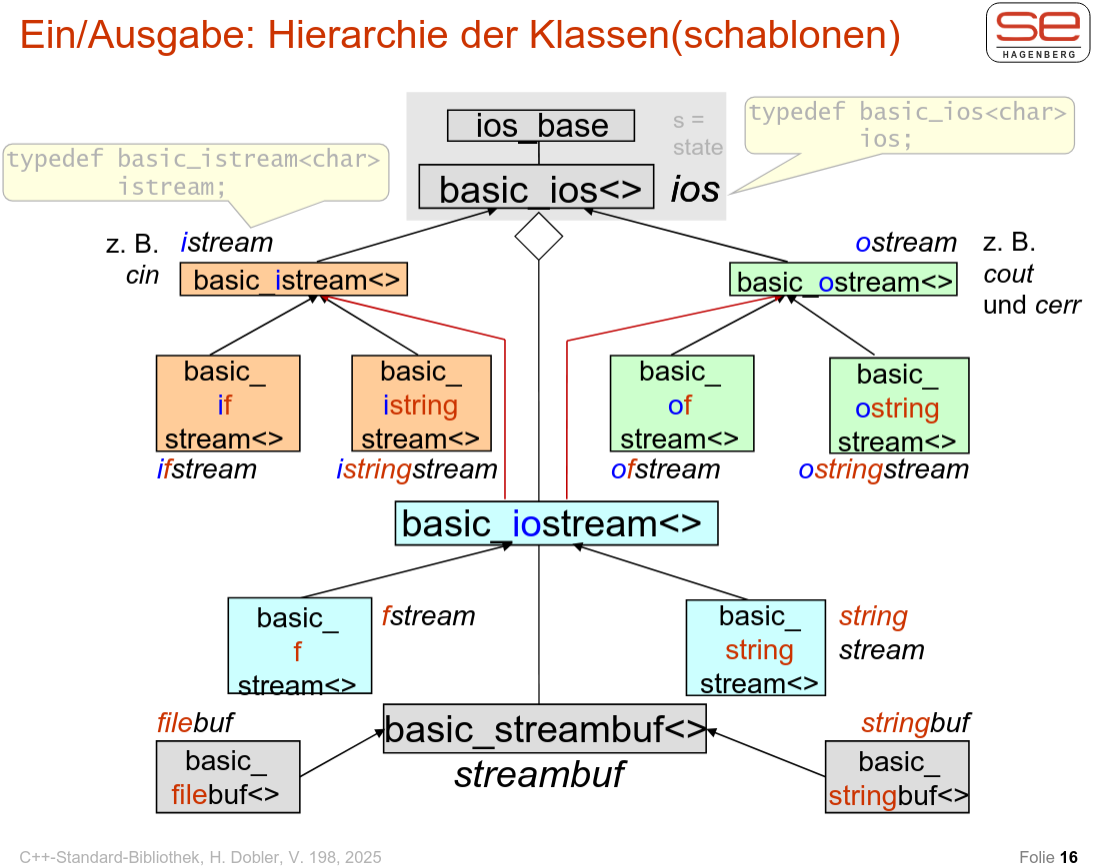
\includegraphics[width=0.45\textwidth]{images/cpp_1.png}
	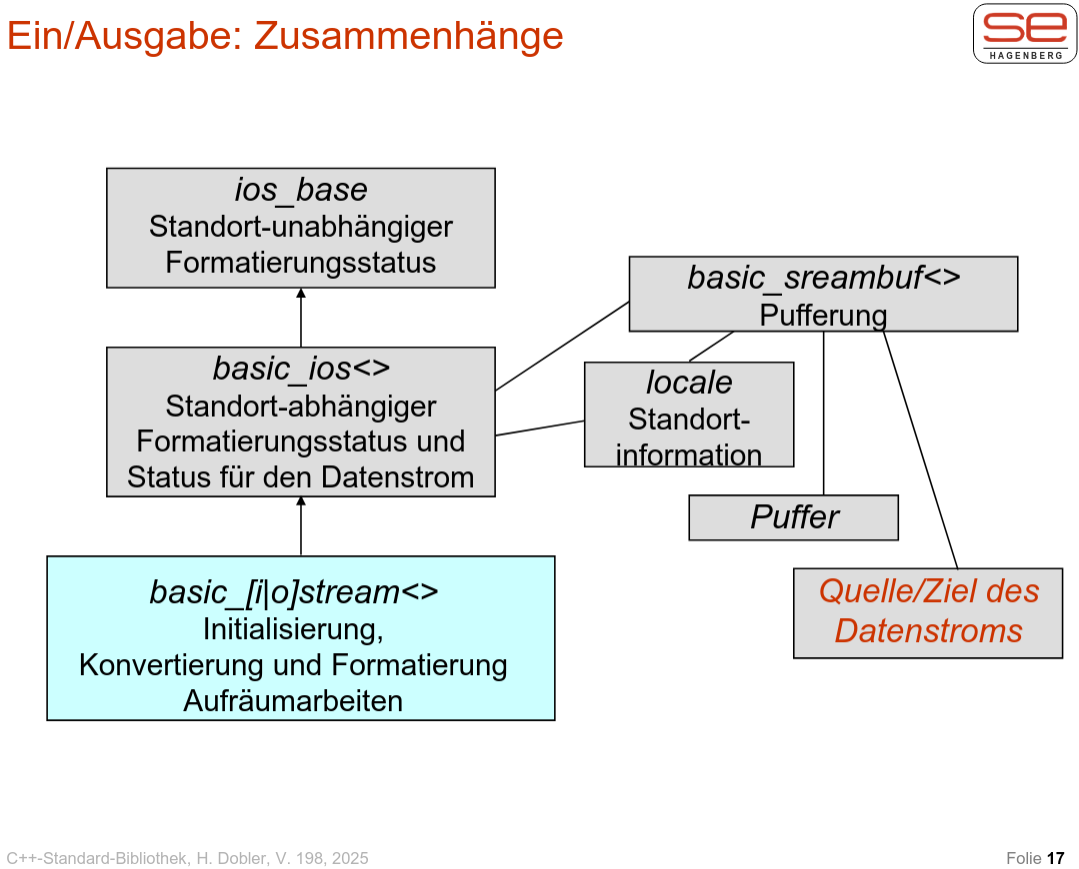
\includegraphics[width=0.45\textwidth]{images/cpp_2.png}
	\caption{Klassenhierarchie der Ein-/Ausgabeklassen in C++}
\end{figure}

Diese Streams sind in mehreren Header-Dateien aufgeteilt:
\begin{itemize}
	\item \textbf{iosfwd} für Vorwärtsdeklarationen(Sehr klein)
	\item \textbf{streambuf} für die Pufferung von Ein-/Ausgabe
	\item \textbf{istream} für die Eingabe
	\item \textbf{ostream} für die Ausgabe
	\item \textbf{iostream} für die Standard-Ein-/Ausgabe
	\item \textbf{fstream} für Dateiein-/ausgabe
	\item \textbf{sstream} für String-Ein-/Ausgabe
	\item \textbf{strstream} für für Char*-Ein-/Ausgabe
	\item \textbf{iomanip} für Ein-/Ausgabeformatierung
\end{itemize}

Flush kann auch mit Stream Aufrufen verkettet werden, z.B. \emph{cout << std::flush;}.
\emph{std::endl} flusht den Stream auch nachdem er einen Zeilenumbruch ausgegeben hat.
Achtung kann Performanceprobleme verursachen, da es den Puffer jedes Mal leert! Wenn mehrere
Zeilenumbrüche ausgegeben werden eher den folgenden Ausschnitt verwenden.

\begin{minted}{cpp}
stream << "\n"
\end{minted}

Es gibt auch diverse Manipulatoren, die das Verhalten von Streams beeinflussen.
\begin{itemize}
	\item \emph{std::dec} für Dezimalzahlen
	\item \emph{std::hex} für Hexadezimalzahlen
	\item \emph{std::oct} für Oktalzahlen
	\item \emph{std::setbase(n)} für die Basis der Zahlendarstellung
	\item \emph{std::setfill(c)} für das Füllzeichen
	\item \emph{std::setprecision(n)} für die Anzahl der Nachkommastellen
	\item \emph{std::setw(n)} für die Breite des Feldes
	\item ...
\end{itemize}

\subsection{STL}
\section{Java}
\subsection{Standard Library}
\subsection{JCF}
\section{Softwaremuster}
\subsection{OOP}
\subsection{Gang of 4}
\subsection{MVC}
\subsection{Iterator}
\subsection{Composite}

\pagebreak
\section{Syntaxvergleich}
Um den Syntax von C++ und Java zu vergleichen, hab ich ein kleines Beispielprogramm geschrieben mit:
\begin{itemize}
	\item einem Interface
	\item einer Basisklasse, die das Interface implementiert
	\item einer abgeleiteten Klasse, die von der Basisklasse erbt
	\item einer Iteratorimplementierung in der abgeleiteten Klasse
	\item einer Main-Methode, die ein Objekt der abgeleiteten Klasse verwendet
\end{itemize}

\subsection{C++}
\subsubsection{Interface}
\inputminted{cpp}{cpp/interface.h}
\subsubsection{Basisklasse}
\inputminted{cpp}{cpp/baseclass.h}
\subsubsection{Abgeleitete Klasse}
\inputminted{cpp}{cpp/derivedclass.h}
\subsubsection{Main}
\inputminted{cpp}{cpp/main.cpp}
\pagebreak

\subsection{Java}
\subsubsection{Interface}
\inputminted{java}{java/src/main/java/javademo/Interface.java}
\subsubsection{Basisklasse}
\inputminted{java}{java/src/main/java/javademo/Baseclass.java}
\subsubsection{Abgeleitete Klasse}
\inputminted{java}{java/src/main/java/javademo/Derivedclass.java}
\subsubsection{Main}
\inputminted{java}{java/src/main/java/javademo/Demo.java}
\pagebreak

% C# kommt nicht zur Klausur
% \subsection{C\#}
% \subsubsection{Interface}
% \inputminted{csharp}{csharp/IInterface.cs}
% \subsubsection{Basisklasse}
% \inputminted{csharp}{csharp/Baseclass.cs}
% \subsubsection{Abgeleitete Klasse}
% \inputminted{csharp}{csharp/Derivedclass.cs}
% \subsubsection{Main}
% \inputminted{csharp}{csharp/Program.cs}
% \pagebreak

\end{document}